\newpage
\section{Anexo: Diagrama P \& ID} \label{anexopid}
	
	
\begin{figure}[h!]
	\centering
	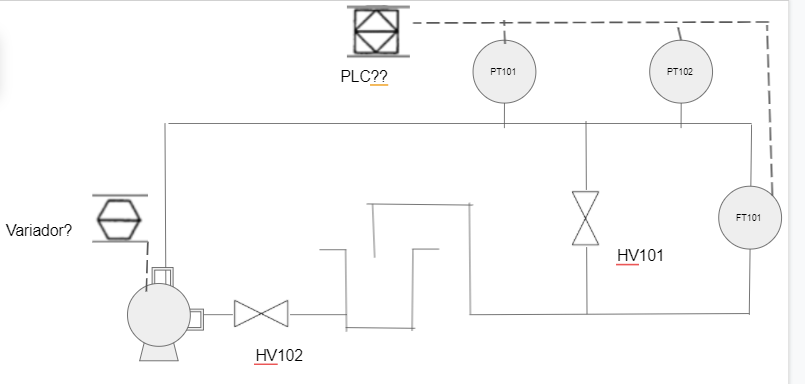
\includegraphics[scale=0.9 ,angle =90]{diag.png}
	\captionof{figure}{Diagrama p\&id}
\end{figure}

\newpage
\section{Anexo: Tabla de Direcciones ModBus} \label{Anexo1}


\begin{longtable}{|p{1.2cm} |p{4cm} |p{4cm} |p{1.5cm} |p{3.2cm} |}
	\caption{Tabla de variables y direcciones}
	\label{tab:direc}  \\
	
	\hline
	\multicolumn{1}{|c|}{\textbf{\begin{tabular}[c]{@{}c@{}}Tipo de \\ variable\end{tabular}}} & \multicolumn{1}{c|}{\textbf{TAG}} & \multicolumn{1}{c|}{\textbf{Descripción}} & \multicolumn{1}{c|}{\textbf{\begin{tabular}[c]{@{}c@{}}Tipo de \\ dato\end{tabular}}} & \multicolumn{1}{c|}{\textbf{Dirección}} \\ \hline
	\endfirsthead
	
	\multicolumn{5}{c}%
	{{\bfseries \tablename\ \thetable{} -- continuación}} \\
	\hline
	\multicolumn{1}{|c|}{\textbf{\begin{tabular}[c]{@{}c@{}}Tipo de \\ variable\end{tabular}}} & \multicolumn{1}{c|}{\textbf{TAG}} & \multicolumn{1}{c|}{\textbf{Descripción}} & \multicolumn{1}{c|}{\textbf{\begin{tabular}[c]{@{}c@{}}Tipo de \\ dato\end{tabular}}} & \multicolumn{1}{c|}{\textbf{Dirección}} \\ \hline
	\endhead
	
	\hline \multicolumn{5}{|r|}{{Sigue en la página siguiente}} \\ \hline
	\endfoot
	
	%\hline \hline
	\endlastfoot
	

	DO & PID\_XSMA0 & Habilitar control automatico manual & Boolean & Device0:000003 \\ \hline
	DO & VSD\_XSM0 & Marcha desde el hdmi & Boolean & Device0:000004 \\ \hline
	DO & VSD\_XST0 & Parada desde SCADA & Boolean & Device0:000005 \\ \hline
	DO & PLC\_XSDES & Desenclave de bomba & Boolean & Device0:000006 \\ \hline
	DO & PID\_XSA0 & PID modo automatico & Boolean & Device0:000008 \\ \hline
	DO & PID\_XSM0 & PID modo manual & Boolean & Device0:000009 \\ \hline
	DO & VSD\_XSFO & Restablecer fallas VSD & Boolean & Device0:000010 \\ \hline
	DI & VSD\_YHS0 & Parada de emergencia fisico & Boolean & Device0:000011 \\ \hline
	DI & VSD\_YLR0 & Modo fisico o scada & Boolean & Device0:000012 \\ \hline
	DI & PID\_YMA0 & Estado manual automatico & Boolean & Device0:000013 \\ \hline
	DI & PID0PIT1\_XRST & Restablecer valores PID & Boolean & Device0:000014 \\ \hline
	DI & PID0PIT2\_XRST & Restablecer valores PID & Boolean & Device0:000015 \\ \hline
	DI & PID0FT1\_XRST & Restablecer valores PID& Boolean & Device0:000016 \\ \hline
	AI & FT01 & Caudal & Float & Device0:400001 \\ \hline
	AI & VSD\_AI1C & Valor del pote & Float & Device0:400003 \\ \hline
	AI & VSD\_IC000 & Corriente & Float & Device0:400005 \\ \hline
	AI & VSD\_SC000 & Frecuencia & Float & Device0:400007 \\ \hline
	AI & VSD\_JC000 & Potencia & UInt & Device0:400009 \\ \hline
	AI & VSD\_WC000 & Torque & UInt & Device0:400011 \\ \hline
	AI & VSD\_EC000 & Voltaje & Float & Device0:400013 \\ \hline
	AI & PIT02 & Presion2 & Float & Device0:400015 \\ \hline
	AI & PIT01 & Presion1 & Float & Device0:400017 \\ \hline
	AI & VSD\_SC001 & Velocidad & UInt & Device0:400019 \\ \hline
	AI & TE001 & Temperatura & Float & Device0:400021 \\ \hline
	AI & PID\_SY000 & Accion de control & Float & Device0:400023 \\ \hline
	AI & VSD\_R\_ERR & Errores, tabla de errores & UInt & Device0:400025 \\ \hline
	AI & PID0PIT1\_TD\_LAG & P1 TD LAG & Float & Device0:400047 \\ \hline
	AI & PID0PIT2\_TD\_LAG & P2 TD LAG & Float & Device0:400049 \\ \hline
	AI & PID0FT1\_TD\_LAG & F1 TD LAG & Float & Device0:400051 \\ \hline
	AI & PID\_SR00 & Valor manual, control desac & Float & Device0:400053 \\ \hline
	AI & PID0PIT1\_SP & Valor Ref P1 & Float & Device0:400057 \\ \hline
	AI & PID0PIT2\_SP & Valor Ref P2 & Float & Device0:400059 \\ \hline
	AI & PID0FT1\_SP & Valor Ref F1 & Float & Device0:400061 \\ \hline
	AI & PID0PIT1\_KI & P1 KI & Float & Device0:400063 \\ \hline
	AI & PID0PIT1\_KP & P1 KP & Float & Device0:400065 \\ \hline
	AI & PID0PIT1\_KD & P1 KD & Float & Device0:400067 \\ \hline
	AI & PID0PIT2\_KI & P2 KI & Float & Device0:400071 \\ \hline
	AI & PID0PIT2\_KP & P2 KP & Float & Device0:400073 \\ \hline
	AI & PID0PIT2\_KD & P2 KD & Float & Device0:400075 \\ \hline
	AI & PID0FT1\_KI & F1 KI & Float & Device0:400077 \\ \hline
	AI & PID0FT1\_KP & F1 KP & Float & Device0:400079 \\ \hline
	AI & PID0FT1\_KD & F1 KD & Float & Device0:400081 \\ \hline
	AI & PID\_SEL & Seleccionar control P1 P2 F1 & UInt & Device0:400083 \\ \hline
	DR & VSD\_ETI & Motor encendido o apagado & Boolean & Device0:400101:4 \\ \hline
	DR & YS\_AP & Alta presion & Boolean & Device0:400103:0 \\ \hline
	DR & YS\_SC & Sin Caudal & Boolean & Device0:400103:1 \\ \hline
	DR & YS\_SP1 & Sin Sensor P1 & Boolean & Device0:400103:2 \\ \hline
	DR & YS\_SP2 & Sin Sensor P2 & Boolean & Device0:400103:3 \\ \hline
	DR & YS\_AT & Alta Temp & Boolean & Device0:400103:4 \\ \hline
	DR & FT01\_YCOM & Sin Caudal & Boolean & Device0:400103:5 \\ \hline
	DR & VSD\_YCOM & Sin comunicación con variador & Boolean & Device0:400103:6 \\ \hline
	%	\\*
	%	\caption{Tabla de variables y direcciones}
	%	\label{tab:direc}  	
	
	
\end{longtable}

\newpage

\section{Anexo: Manual BANCO-SCADA}
\subsection{Características generales}
\begin{itemize}
	\item Para sistemas operativos Windows 7 y Windows 10.
	\item Se puede utilizar el banco de pruebas en modo local o remoto.
	\item Diseñado para controlar tres variables distintas, dos de presión o caudal.
		\item Fácil de transportar.
	\item Posibilidad de generar perturbaciones en el sistema para observar distintas respuestas.
\item Posibilidad de guardar valores históricos y ver datos en tiempo real.
\end{itemize}


\subsection{Guía de uso}
\begin{enumerate}
	\item Conectar el banco de pruebas con los respectivos sensores y transmisores en el módulo correspondiente del PLC.
	\item Conectar cable Ethernet entre PLC y router o PC.
	\item Alimentar el sistema del variador con tensión trifásica y la fuente del PLC con tensión monofásica.
	\item Verificar que los dispositivos se encuentren en la misma red.
	\item Abrir iFix, la base de datos y el\textit{ driver MBE} dónde se procederá a conectar el sistema SCADA. 

	\item Comprobar comunicación al ejecutar la pantalla SCADA.
\end{enumerate}

\subsubsection{Pantalla principal}
En la figura \ref{fig:pantalla1} se observa la pantalla principal del SCADA y en la figura \ref{fig:partes} se divide en varias secciones.

\begin{figure}[h!]
	\centering
	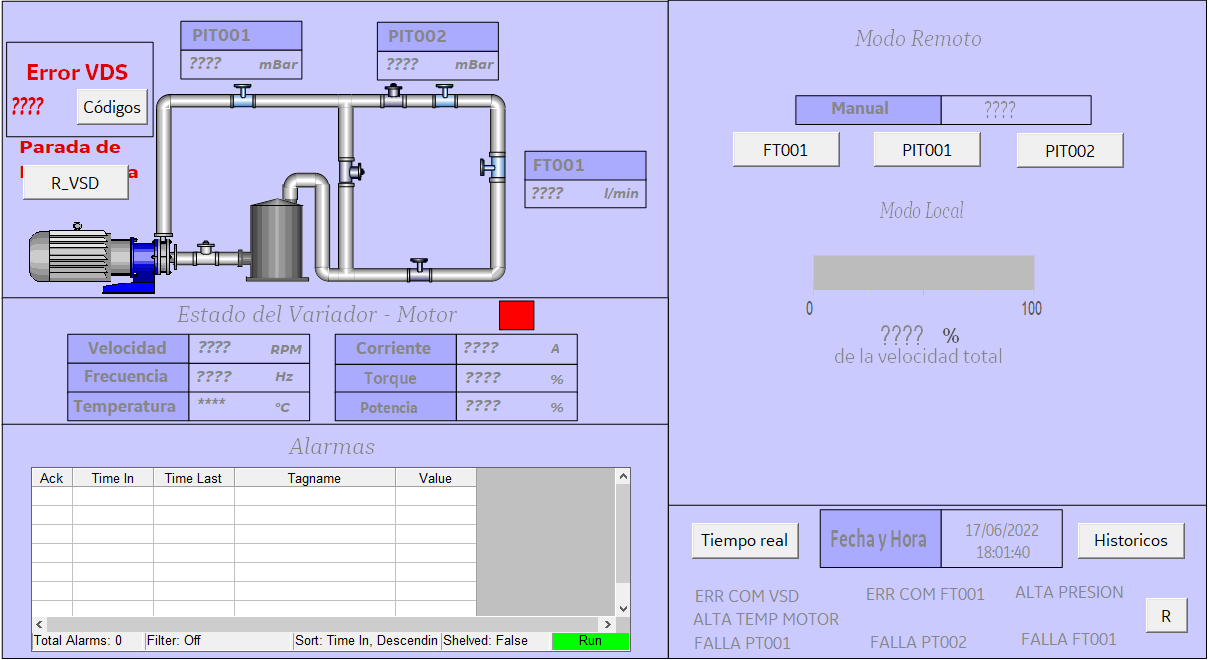
\includegraphics[width=0.9\linewidth]{pantalla1.png}
	\captionof{figure}{Pantalla principal}
	\label{fig:pantalla1}
\end{figure}
\begin{figure}[h!]
	\centering
	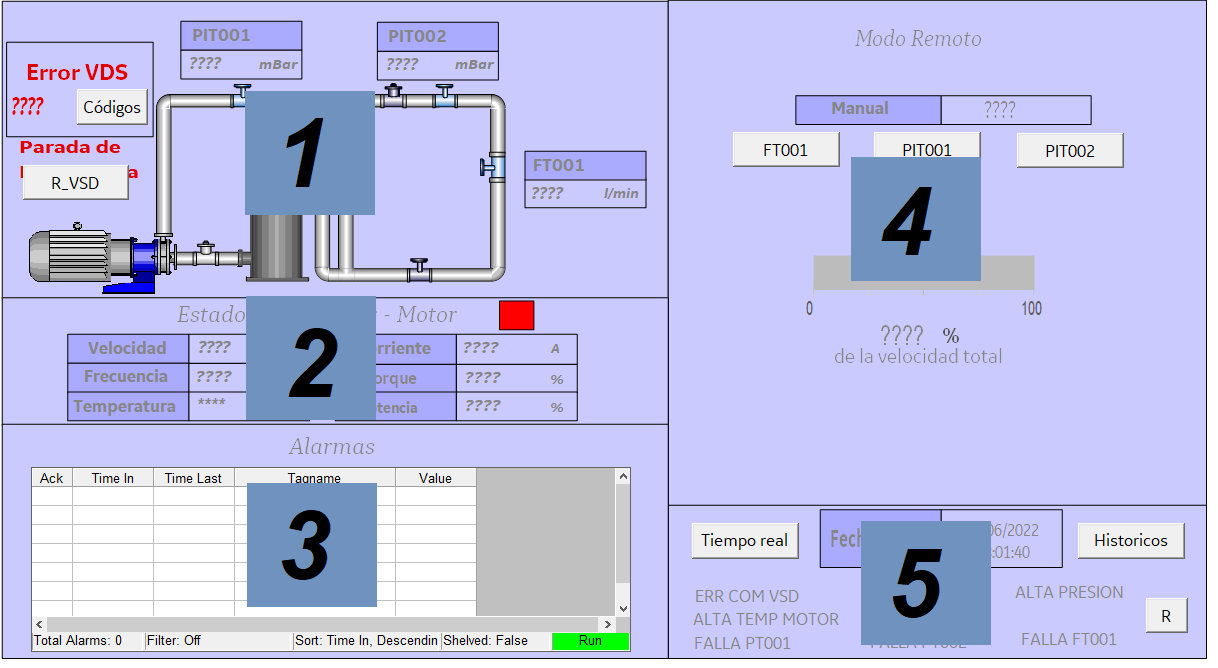
\includegraphics[width=0.6\linewidth]{p_partes.png}
	\captionof{figure}{Partes del sistema SCADA}
	\label{fig:partes}
\end{figure}

\paragraph{Diagrama del banco de pruebas}
Se observan los valores de presión y caudal en un diagrama similar al banco de pruebas físico.

En caso de ocurrir un error sobre el VSD, se observará el código del lado izquierdo (A), a su vez al presionar sobre el botón \textit{Códigos} se mostrará la tabla de errores. Si se desea reconocer el error se debe presionar el botón B (Figura \ref{fig:pp1}).
\begin{figure}[h!]
	\centering
	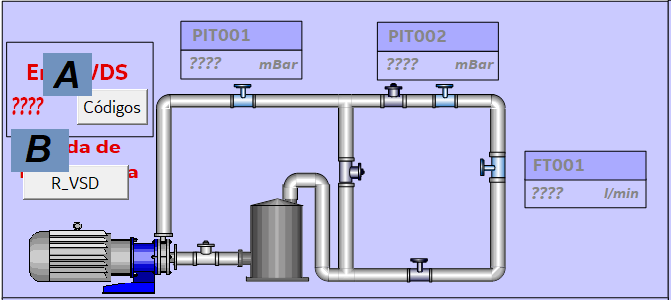
\includegraphics[width=0.6\linewidth]{p_p1.png}
	\captionof{figure}{Subpantalla 1}
	\label{fig:pp1}
\end{figure}

También en la parte izquierda de la pantalla, se mostrará la indicación de parada de emergencia física.

\paragraph{Estado del variador - Motor}
En esta sección se ve una señal piloto de color rojo, si es que el motor se encuentra en funcionamiento, lo que indica señal de cuidado o alerta; mientras que en color verde si el motor está apagado. Se observan variables de velocidad y frecuencia del motor, temperatura obtenida por el RTD y corriente, torque y potencia consumida por el motor.
\paragraph{Alarmas}
Sección destinada al alarmero dónde muestra el período de tiempo que ocurrió el hecho, el nombre de la variable y el valor alcanzado.
\paragraph{Modo remoto/ Modo local}
\begin{itemize}
	\item Modo Local
	
	Si la llave selectora del banco de pruebas se encuentra en modo local, se observará el cartel que indica \textit{Modo Local} (Figura \ref{fig:localremoto}.a).
	
	\item Modo Remoto
	
	Si la llave selectora del banco de pruebas se encuentra en modo remoto, el sistema está preparado para recibir órdenes desde SCADA. El motor puede encenderse con velocidad 0 al presionar la tecla A o encender a una velocidad preestablecida fijada previamente con un valor entero en RPM entre 0 y 3600 (Figura \ref{fig:localremoto}.b). 
	
	Si desea se puede abrir cada ventana del lazo de control (Figura \ref{fig:LC}) ``botones B'' dónde muestra el valor de cada constante del PID, se puede colocar otros valores mientras que se use la coma como separador decimal. Con el ``botón C'', se podrá restablecer los valores del PID cuyos valores fueron fijados al momento de realizar el proyecto (Tabla \ref{tab:pid2}).
	
	\begin{table}[h]
		\centering
		\begin{tabular}{|l|l|l|l|}
			\hline
			& PIT01 & PIT02 & FT01 \\ \hline
			$K_p$ & 3,05 & 5,453 & 104,3 \\ \hline
			$K_i$ & 0,396 & 0,348 & 0,719 \\ \hline
			$K_d$ & 0 & 0 & 0 \\ \hline
			N & 1000 & 1000 & 1000 \\ \hline
		\end{tabular}
		\captionof{table}{Valores de los PID}
		\label{tab:pid2}
	\end{table}
	
		
	Al colocar el selector en automático (D), se cierra el lazo del sistema y puede establecerse la presión o caudal deseado en ``E'' y los rangos serán establecidos según la tabla \ref{tab:rang}. En caso de que se encuentre el selector en manual (D) los valores se establecerán según la entrada de valor \textit{Manual} en RPM del motor. (Figura \ref{fig:localremoto}.b). 
\end{itemize}

\begin{figure}[htbp]
	\centering
	\subfigure[Modo local]{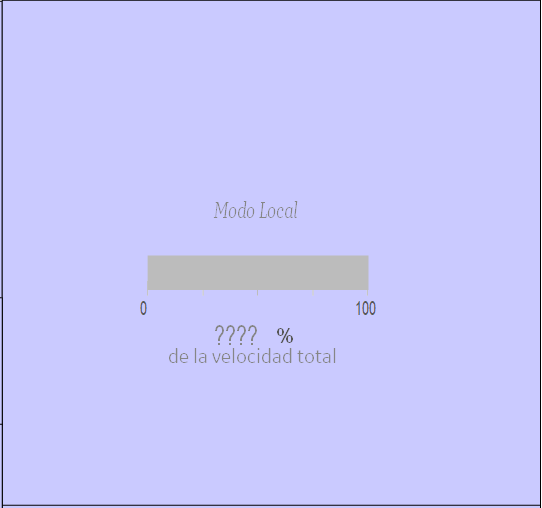
\includegraphics[width=60mm]{p_4c.png}}
	\subfigure[Modo remoto]{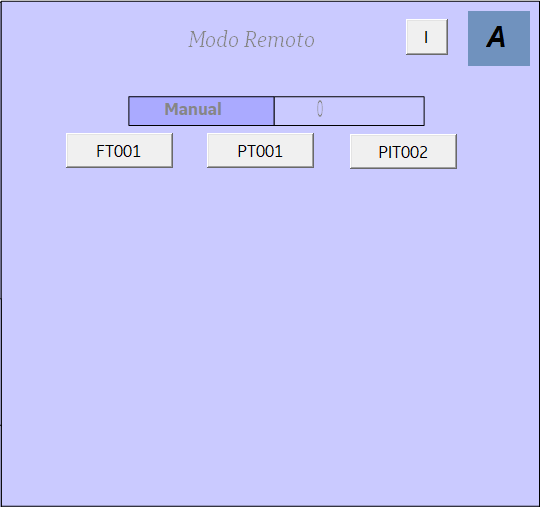
\includegraphics[width=60mm]{p_4b.png}}
	\caption{Subpantalla 4} \label{fig:localremoto}
\end{figure}

\begin{figure}[h!]
	\centering
	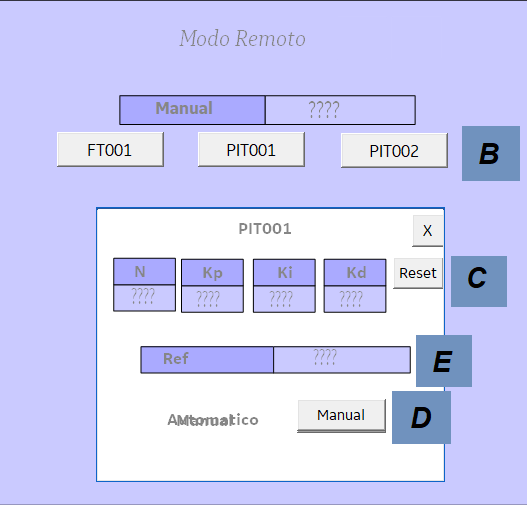
\includegraphics[width=60mm]{p_4a.png}
	\captionof{figure}{Modo lazo cerrado}
	\label{fig:LC}
\end{figure}
\begin{table}[]
	\centering
	
	\begin{tabular}{|cc|l|c|}
		\hline
		\multicolumn{2}{|l|}{\textbf{Variable}} & \textbf{Rango} & \multicolumn{1}{l|}{\textbf{Unidades}} \\ \hline
		\multicolumn{1}{|c|}{\textbf{PIT001}} & Presión & 60 - 930 & mbar \\ \hline
		\multicolumn{1}{|c|}{\textbf{PIT002}} & Presión & 60 - 700 & mbar \\ \hline
		\multicolumn{1}{|c|}{\textbf{FT001}} & Caudal & 2 - 11,7 & l/min \\ \hline
	\end{tabular}
\caption{Rangos de las variables}
\label{tab:rang}
\end{table}

\paragraph{Fallas y ventanas de gráficos}
En la pantalla 5 se observan los carteles de eventuales fallas que puedan ocurrir en el sistema, y se pueden reanudar con el botón \textit{R}.

Otra de las cosas que tiene esta subpantalla es la fecha, hora y dos botones dónde al presionarlos se abren pantallas para observar gráficamente datos en tiempo real o de forma histórica (Sección \ref{sec:graf} y \ref{sec:graf2}).

\subsubsection{Pantalla de datos en tiempo real} \label{sec:graf}
En la figura \ref{fig:scadaTR} se puede observar la pantalla con valores instantáneos (la imagen no corresponde a valores reales tomados durante las pruebas).
\begin{figure}[h!]
	\centering
	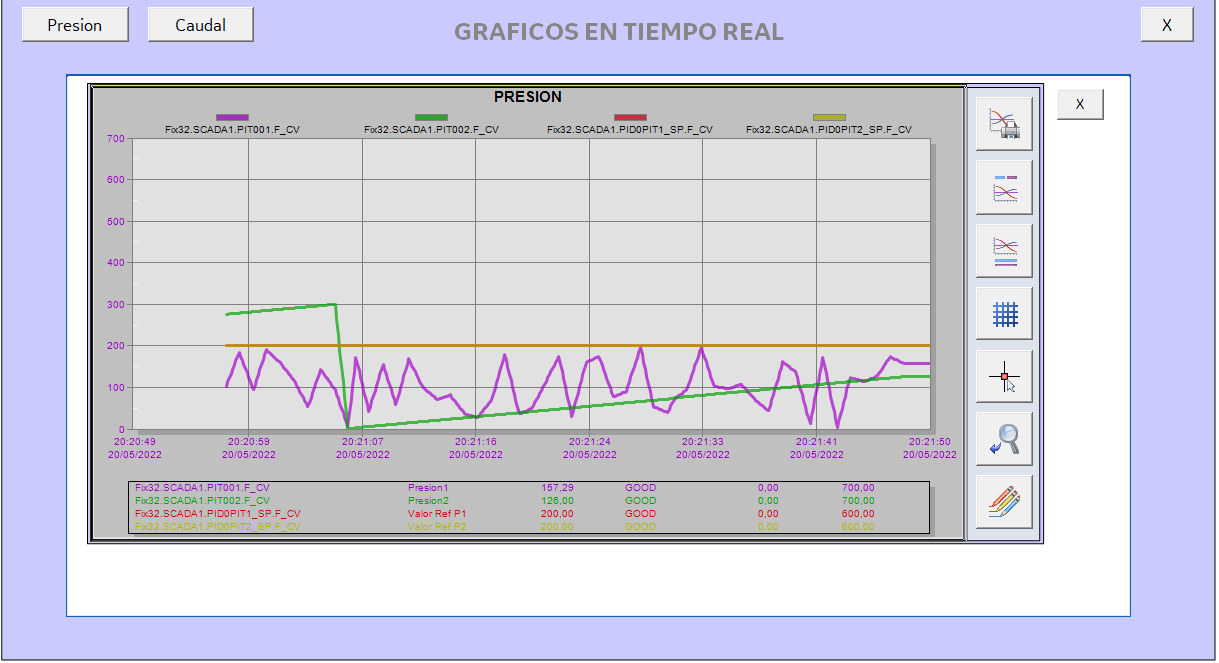
\includegraphics[width=1\linewidth]{scadaTR.png}
	\captionof{figure}{Pantalla de datos en tiempo real}
	\label{fig:scadaTR}
\end{figure}

\subsubsection{Pantalla de datos históricos} \label{sec:graf2}
Para la interpretación de datos históricos se puede realizar de dos formas, una es crear un archivo .txt y la otra es de forma gráfica. 

Para observar los datos históricos en el gráfico de tiempo, se debe presionar alguna opción de los botones superiores izquierdos, además se selecciona el período de tiempo que se desea visualizar (Figura \ref{fig:scada3a3}.b).

Para generar el archivo \textit{.txt} con los valores históricos se presiona el botón \textit{Exportar}, se conecta con el servidor Historian y se selecciona las variables de interés con el período que se quiera guardar.
Finalmente se le asigna un nombre al archivo y se presiona \textit{Export} (Figura \ref{fig:scada3a3}.a).


\begin{figure}[htbp]
	\centering
	\subfigure[Pantalla para guardar datos históricos]{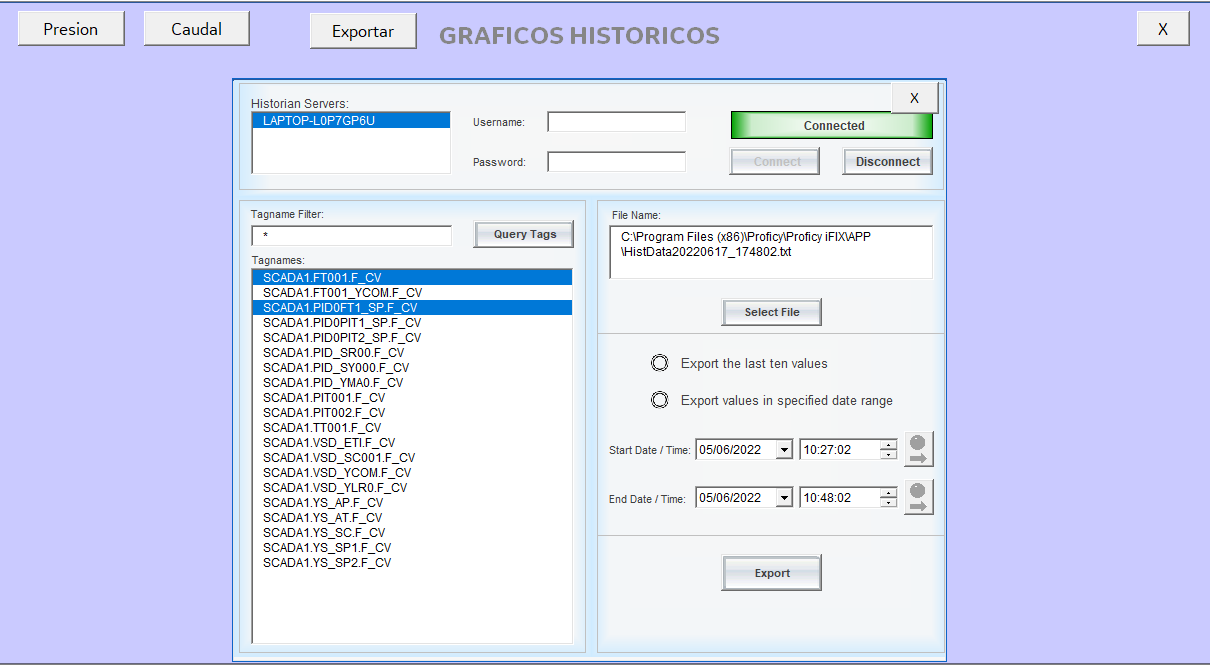
\includegraphics[width=1\linewidth]{scada33.png}}
	\subfigure[Datos históricos de forma gráfica]{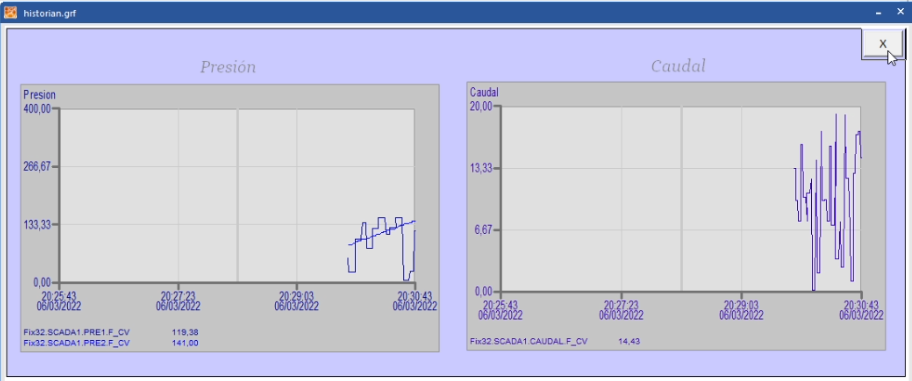
\includegraphics[width=1\linewidth]{scada3.png}}
	\caption{Datos históricos} \label{fig:scada3a3}
\end{figure}



\newpage